\chapter{Scope rules}\label{chap:scope-rules}
This section describese scope rules and the environment-store model for the language. It is important to know how the values of variables are being stored as well as knowing how the language handles encapsulation. 

\section{The environment-store model}\label{sec:es-model}
It is important to know how the environment-store model works, because the model describes how variables contents are stored, and what location a variable is bound to. Furthermore it also describes what content a location has stored. Figure \ref{fig:esmodel}, illustrates the environment-store model. The model shows contains three boxes. The left box is the environment, the middle is the location and the right is the store. The environment is the variables. A variable is bound to a location, which is illustrated by the arrow, $env_v$, connecting the \textbf{environment} and \textbf{location}. $env_v$ is a function that retrieves the location of a variable. The content of a variable can be stored on a location, which is illustrated by the $sto$ arrow, connecting \textbf{location} and \textbf{store}. $sto$ is a function that retrieves the content stored on a location. 

\\For example, the model shows that the variable $x$ is bound to location $l_{1}$, which has the value $5$ stored. The same is valid for the variables $y$ and $z$, which are bound to $l_{2}$. However these two variables are bound to the same location, which has the same value stored. If for example, the value 13 in store, gets changed to 15, then the value for both variables $y$ and $z$ changes. 
\todo{Matti: Ændrer navnene på locations til l1, l2}
\begin{figure}[H]
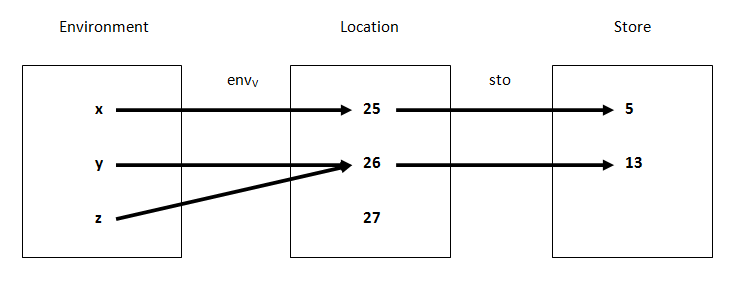
\includegraphics{billeder/environment_store_model.png}
\caption{Environment-store model}
\label{fig:esmodel}
\end{figure}


\section{The scope rules}\label{sec:scope-rules}




\begin{center}
\begin{tabular}{ l l}
\hline
& \\
$[CALL-STAT-STAT_{BSS}]$ & $env'_{v}~[next \rightarrow l], env'_{p}~ \vdash \langle S,sto \rangle \rightarrow sto' \over env_{v}, ~ env_{p} \vdash \langle call~p, sto \rangle \rightarrow sto'$ \\
& where $env_{p}p = (S,env'{v},env'{p})$ \\
& and $l = env_{v}next$ \\
\hline
\end{tabular}
\end{center}







